\documentclass[12pt]{article}
\usepackage[margin=1.in]{geometry}
\usepackage[utf8]{inputenc}
\usepackage[T1]{fontenc}
\usepackage{booktabs,nicefrac,microtype}
\usepackage{lmodern}

\usepackage{xcolor}
\definecolor{linkblue}{rgb}{0.1,0.4,0.7} %blue
\usepackage[colorlinks=true,citecolor=linkblue]{hyperref}
\usepackage{multibib}
\usepackage{natbib}
\usepackage{multicol}
\usepackage{physics}
\usepackage{amsfonts,amsmath,amsthm,amssymb}
\usepackage{mathtools}
\usepackage{wrapfig}
\usepackage{pifont}

\newcommand{\cmark}{ \textcolor{green!60!black}{\ding{51}} }
\newcommand{\xmark}{ \textcolor{red!60!black}{\ding{55}} }
\usepackage{wrapfig}

\usepackage{colortbl}
\usepackage{tabularx}
\usepackage{graphbox}
\usepackage{graphicx}
\usepackage{comment}
\usepackage{xurl}
\usepackage{multirow}
\usepackage{booktabs}
\usepackage{algorithm, algpseudocode, algcompatible}
\usepackage{footmisc}
\usepackage{caption}
\usepackage{subcaption}

\newcommand{\orange}[1]{\textcolor{orange}{#1}}
\newcommand{\red}[1]{\textcolor{darkred}{#1}}
\newcommand{\green}[1]{\textcolor{cadmiumgreen}{#1}}




\usepackage{tikz}
\usetikzlibrary{decorations.pathreplacing}
\usetikzlibrary{fadings}


\title{Sleep stage estimation using RNNs with physiological data from wearable devices}
\author{}
\begin{document}
\maketitle



\section{Introduction}
% Importance of sleep and sleep analysis
On average an individual spends about one-third of their life in sleep. Sleep is vital for effective functioning and health in humans. Getting adequate sleep every day can help one maintain/improve mental, physical health, and overall quality of life. On the other hand, lack of sleep can lead to problems such as difficulty in decision making,  emotional imbalance; persistent sleep deprivation is associated with a higher risk of chronic health problems. In a nutshell, good sleep is important for a healthy lifestyle in humans. 


% Sleep tracking and estimation
% Current trends in personal sleep montoring
The last decade has seen tremendous growth in the popularity of consumer wearable devices. At the same time, there is also an increasing emphasis on tracking personal health metrics. Sleep tracking is one such aspect with implications on overall health and lifestyle quality. Currently, there are many products in the consumer wearables market aimed at measuring sleep quality and efficiency \citep{shelgikar2016sleep}. These devices typically collect numerous data from multiple sensors such as heart rates, movements, body temperature, among others.  Subsequently, various factors such as sleep stages, sleeping timings, latency are considered while estimating the overall sleep quality and efficiency for end consumers. 


In most wearable technologies, the underlying algorithm is undisclosed and the access to all the metadata considered by the algorithm is restricted. The reliability of these metrics given by the devices is also questionable in many cases \citep{kolla2016consumer}.  Therefore, this project aims to study the feasibility of estimating sleep stages based on the observations made by wearable devices.  In particular, we consider the problem of estimating sleep stages based on heart rate and movement metrics, commonly measured with many wearable devices.  



We consider the open-source data available on \url{physionet.org} \footnote{\label{dataurl}\url{https://physionet.org/content/sleep-accel/1.0.0/}} reporting personal activity, physiological observations, and sleep stage measurements. We closely follow the accompanying approach proposed by the authors responsible for open-sourcing the data  \citep{walch2019}, and empirically evaluate different algorithms to address the sleep stage estimation problem. The prior work of \cite{walch2019} explored sleep stage classification based on epochs of 30 seconds in isolation. This previous work considered classification techniques such as random forests, k-nearest neighbors, logistic regression treating every epoch independently over time. This independence over time assumption can be restrictive as it ignores temporal correlations in the data.  In the current work, we considered state-space methods using RNNs that can model the temporal structure of the data. The more recent works on the sleep estimation problem also considered deep neural network based approaches  \citep{biswal2018expert,radha2019sleep,haghayegh2021deep}, however on datasets based on heart rate variability measurements that are different than the one under study . With the proposed RNN model, we observed around 10\% increase in classification performance. Empirically, we observed that we can estimate different sleep stages based on heart rate and motion measurements with around 70\% accuracy. 


\begin{figure}
\centering
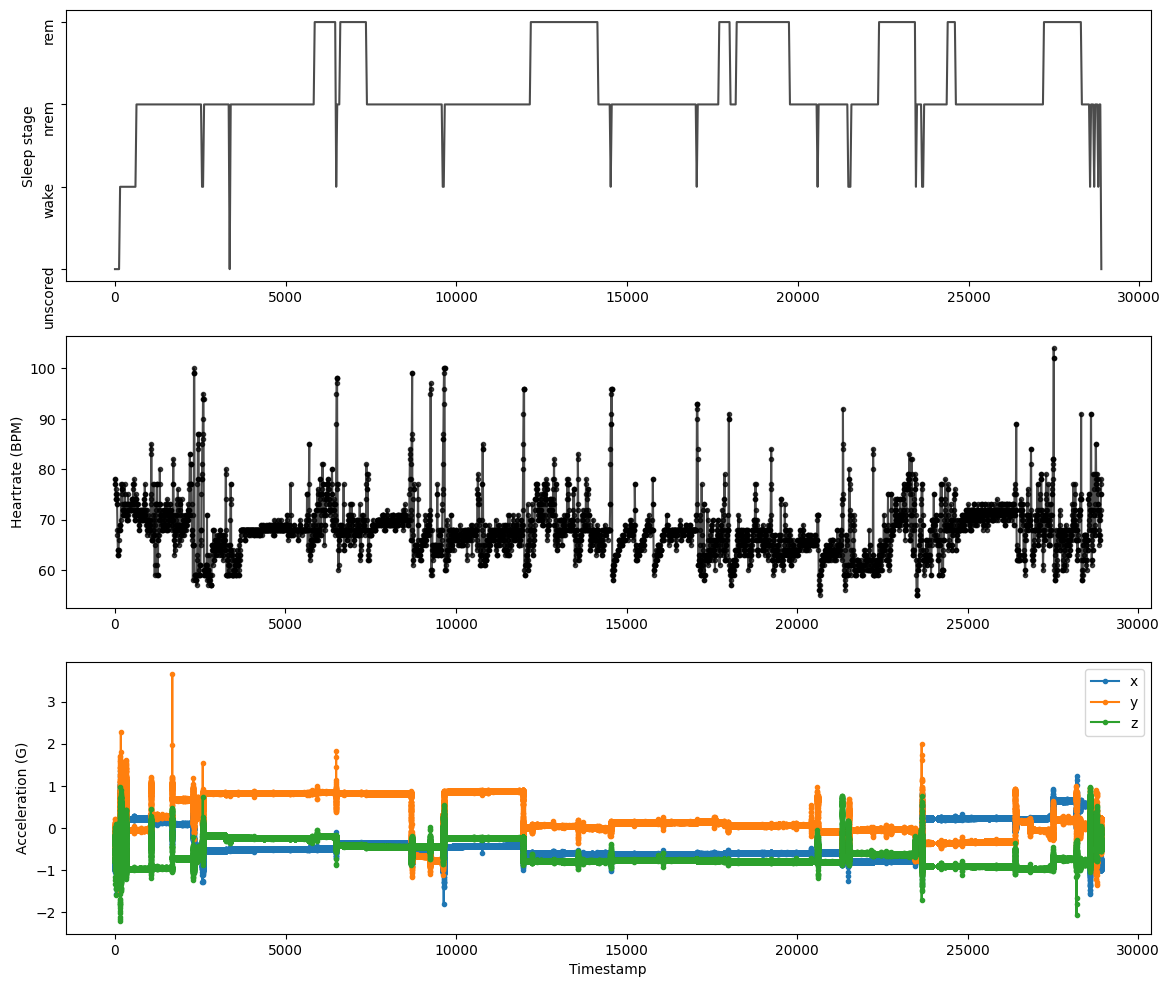
\includegraphics[width=\textwidth]{figures/8000685_cropped.png}
\caption{Visualization of the raw data for subject \texttt{8000685}. The dataset consists of sleep stage labels tagged at 30 second epochs. In addition, the heart rate and acceleration parameters are measured at irregular time intervals.}
\label{fig:8000685_cropped}
\end{figure}


\section{Problem formulation}
% Sleep stage description, what every stage means, how it is measured
Normal sleep in a healthy individual comprises two different stages: rapid eye movement (REM), and non-rapid eye movement (NREM). One sleep episode typically consists of alternating cycles through the REM and NREM sleep stages, along with possible wakefulness states in between. The NREM stage can be further divided into four stages N1, N2, N3, and N4, with N1 \& N2 typically considered ``light sleep''  and N3 \& N4 ``deep sleep'' states. Characterization of good sleep in an individual requires an understanding of personal sleep stage progression.  The currently established gold standard for sleep measurement is the polysomnogram (PSG). However, quantifying sleep with PSG is an expensive process, as it requires measuring multiple physiological parameters in a sleep laboratory \citep{berry2015aasm}. More accessible ways of measuring sleep can be helpful for wider utilization of sleep medicine, which can bring health and lifestyle improvements for many people.



Given the difficulty in large-scale usage of polysomnography for personal sleep tracking, estimating sleep using other consumer wearable devices can be a convenient solution. Such wearable devices are commonly affordable, track multiple personal biological signals, and adopted by the wider population over recent years. In the context of sleep tracking, measurements of motion with accelerometers, heart rate, and respiratory signals with photoplethysmography (PPG), body temperature measurements can be useful. Such parameter tracking is available in many wearable devices today. Such variables measured can be thought to have a predictive relationship with the sleep stages. In this project, we consider the problem of estimating sleep stages using data regarding heart rate and motion variables with different machine learning predictive modeling techniques. 



Sleep data can be thought of as a dynamic process, with temporal structure in place. In particular, there are specific patterns generated at different sleep stages regarding the measurable variables, which can be utilized for predictive modeling. In specific, we consider heart rate and motion as measurables that can have explicit patterns in NREM/REM/ Wake states in a typical sleep episode. Hence, we can treat the sleep stage estimation problem as a classification problem with observed measurements as input variables and gold-standard sleep stage labels from PSG as target variables. Given that we can build such a model with good accuracy, we can utilize such a model for estimating sleep stages for a general population using wearable devices.  


\section{Dataset description}
\subsection{Data generation}
The dataset used in this work consists of the data recorded for 31 subjects at the University of Michigan as part of the work by \citet{walch2019}.  The sleeping data for all the subjects were recorded with PSG over a course of one night with an opportunity to sleep for 8 hours. The subjects were also asked to wear Apple Watch (Apple Inc.) while undergoing PSG recording. The Apple watch was used to record motion data with MEMS accelerometers and heart rate data with photoplethysmography (PPG). \citet{walch2019} also provide an open-source codebase for accessing heart rate and accelerometer data from Apple watch \footnote{\url{https://github.com/ojwalch/sleep_accel}}. 


\subsection{Raw dataset}
The raw dataset consists of true sleep stages over time as recorded by PSG along with the motion and heart rate data over time, for the duration of one night.

\paragraph{Sleep stage data with PSG}
The dataset consists of sleep stage measurements for 31 subjects using PSG. Each subject can have a possibly different sequence length based on their sleep duration on the night of study. These sleep stages consist of 6 labels: REM, N1, N2, N3, N4, Wake, and Unscored. The PSG labels were recorded by considering measurements of multiple biological signals using electroencephalogram (EEG), electrooculogram (EOG), electrocardiogram (ECG), among others following the technical specifications of the American Academy of Sleep Medicine (AASM) \citep{berry2015aasm} in the laboratory. We refer readers to \citet{walch2019} for further information on the PSG recording process. 


\paragraph{Heart rate and motion data} In addition to the sleep stage labels, the heart rate data in beats per minute (BPM) and motion data in units of $g$ ($9.8 m/s^2$) using Apple watch. The motion data consists of accelerometer reading in $x$, $y$, and $z$ directions. Both heart rate and acceleration data are measured at irregular time intervals as shown in Figure \ref{fig:8000685_cropped}. 


\begin{figure}
\centering
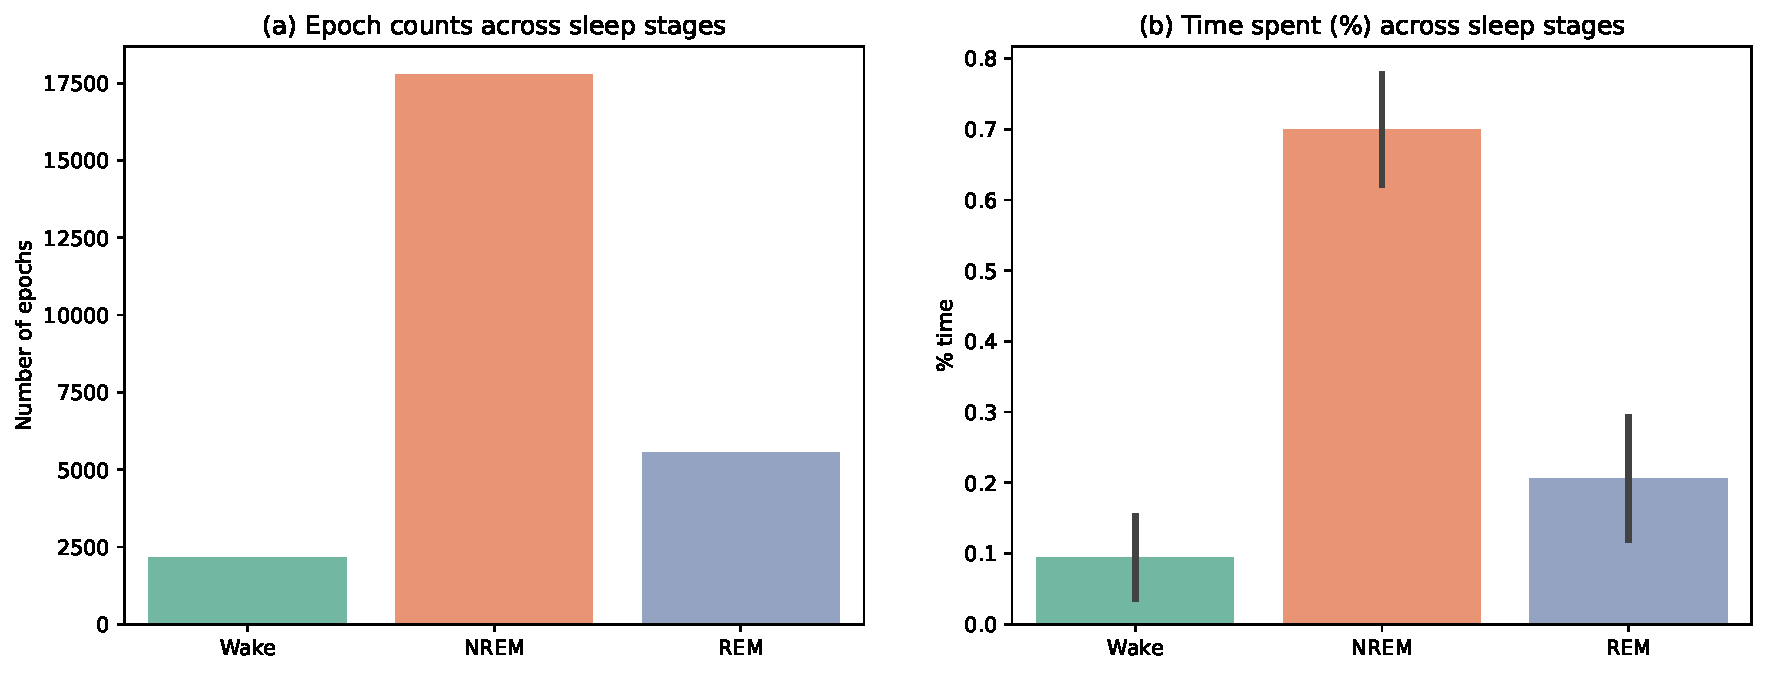
\includegraphics[width=\textwidth]{figures/histogram_sleep_counts.pdf}
\caption{The modeling dataset consists of three classification labels : NREM, REM and Wake. Around 70\% of epochs or observations are od NREM stage, followed by around 20\% of REM, and around 10\% of Wake states as shown in subplot (a). The CI in subplot (b) shows the variation across subjects : the subject-level sleep distribution is similar to the population-level distribution. This observation is consistent with the general understanding of sleep \citep{carskadon2005normal}.}
\label{fig:histogram_sleep_counts}
\end{figure}


\subsection{Modeling dataset}
\label{sec:modeling_dataset}
\paragraph{Classification targets} The raw dataset consists of six sleep stage labels (REM, N1-N4, Wake) along with an additional ``Unscored'' label. These PSG labels are generated for every 30 second time interval called ``epochs''. The raw dataset was filtered to exclude the ``Unscored'' epochs while generating the modeling dataset. In addition, the four sleep stages N1-N4 were combined to form the NREM stage for classification modeling target with three classes: REM, NREM, and Wake stages.



The population-level histogram or marginal distribution of the sleep stage labels are shown in Figure \ref{fig:histogram_sleep_counts}. The distribution is not uniform across different labels as shown in the figure. NREM is the majority class covering around 70\% epochs, followed by REM of 20\% and Wake state around 10\%. This indicates that the class imbalance needs to be carefully considered while building the classification model. 


\begin{figure}
\centering
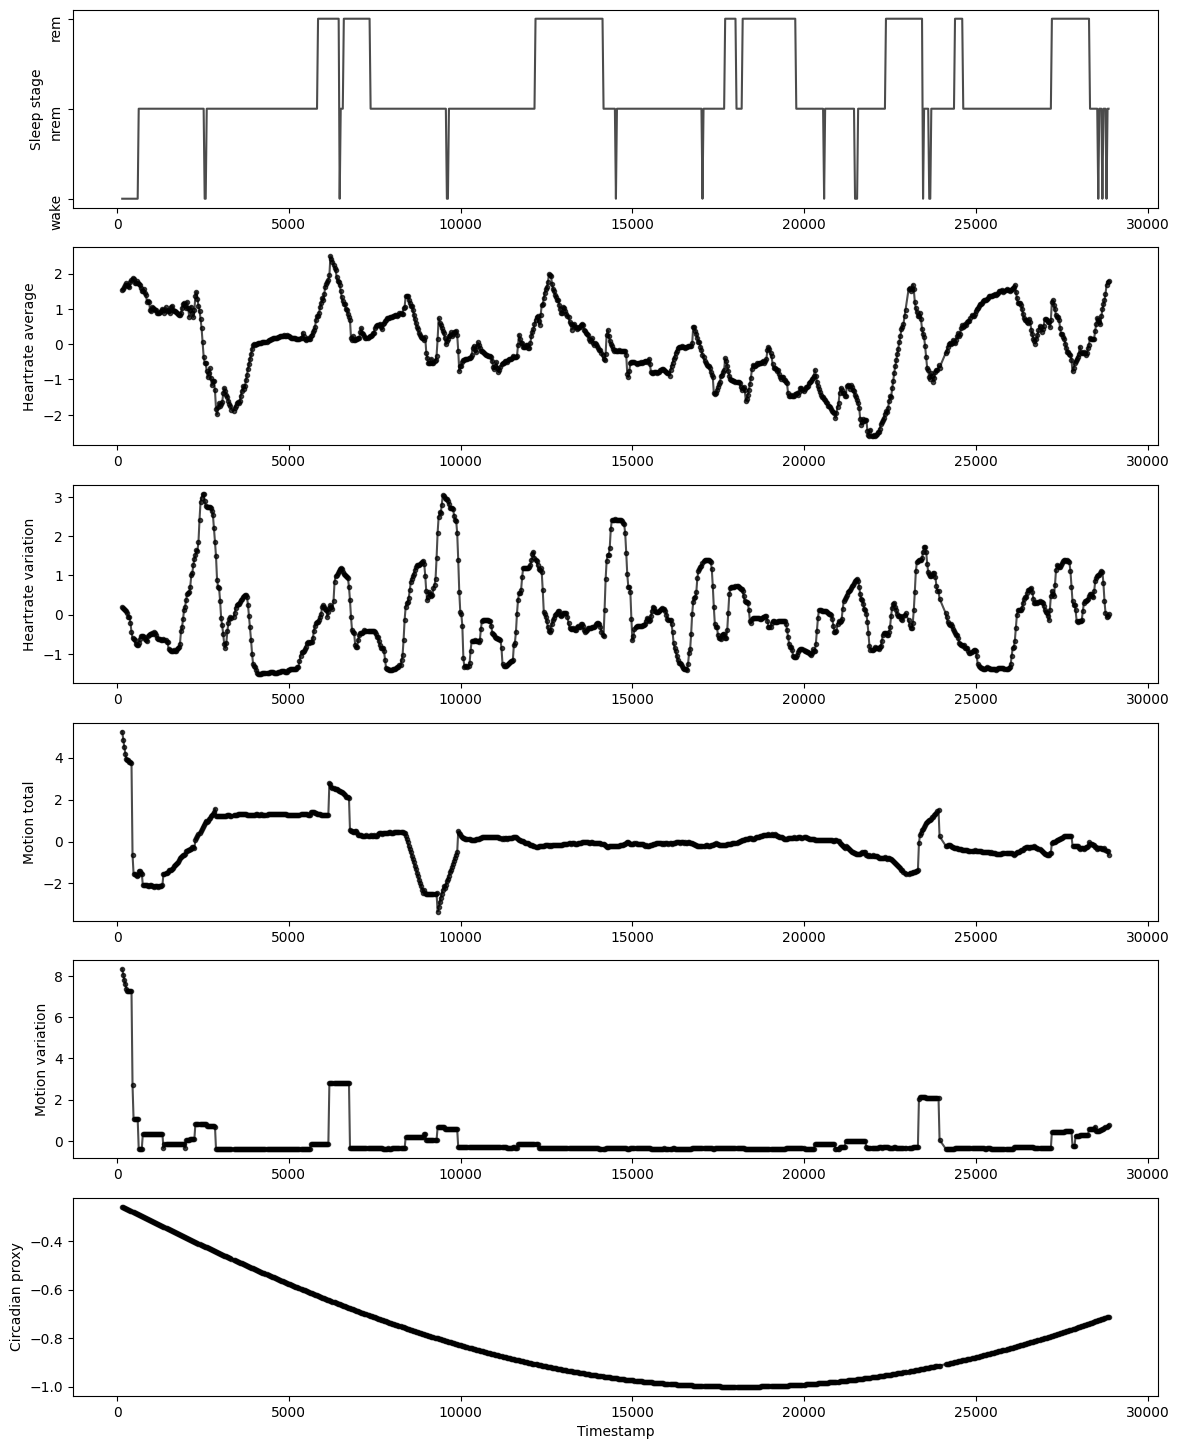
\includegraphics[width=\textwidth]{figures/8000685_features.png}
\caption{Visualization of the modeling features for subject \texttt{8000685}. The modeling dataset consists of sleep stage labels at regular 30 second epochs. The input features consists of two heart rate related features: average heart rate and heart rate variation, two motion related features: average motion and motion variation, and a time-based circadian proxy feature.}
\label{fig:8000685_features}
\end{figure}

\paragraph{Classification inputs}
While the PSG labels are recorded in regular 30-second epochs,  the motion and heart rate (HR) data are recorded from Apple watch at irregular time intervals. As a preprocessing step, these irregular HR and motion data were interpolated to one-second intervals for every subject. This resulted in each sleep epoch having 30 measurements of HR and motion data respectively. The 30 measurements for every epoch were further aggregated to produce different modeling input features as described below.


The HR readings were aggregated to two different features (1) average HR feature, and (2) HR variation feature. Average HR corresponds to the mean HR value for the 30-second epoch interval. The HR variational corresponds to the standard deviation of the heart rate differentials generated by convolving the interpolated HR signal with 120 second and 600-second difference of Gaussian filters. 


The motion readings were also aggregated to two different features (1) average motion feature, and (2) motion variation feature. These features are computed as mean and standard deviation values of total motion (defined as squared L2 norm) of interpolated accelerations in the 30-second epoch intervals.  


The physiological variables such as HR and motion can be considered as observable responses of underlying sleep states in subjects. While such variables could help build a predictive model, we could also consider the external environmental influence on an individual's sleep. Such external variables can be considered under a 24-hour cycle referred to as the ``circadian cycle'' that can indicate sleep propensity in individuals. In this work, we follow the approach of \cite{walch2019} and include an additional time-based feature that maps the clock-time to a cosine signal for individual sleep episodes as shown in Figure \ref{fig:8000685_features}.




\section{Methods}
\subsection{Baseline models} In the work accompanying the dataset under study, \citet{walch2019} proposed classification models for sleep stage prediction using acceleration and heart rate measurements. The modeling formulation in this work treated every sleep epoch in isolation. Specifically, this prior work explored models such as random forests, logistic regression and provided an open-source codebase \footnote{\url{https://github.com/ojwalch/sleep_classifiers/}}. In this work, we trained models similar to \citet{walch2019} as baselines on the modeling dataset described in Section \ref{sec:modeling_dataset}.




%\begin{figure}
%\centering
%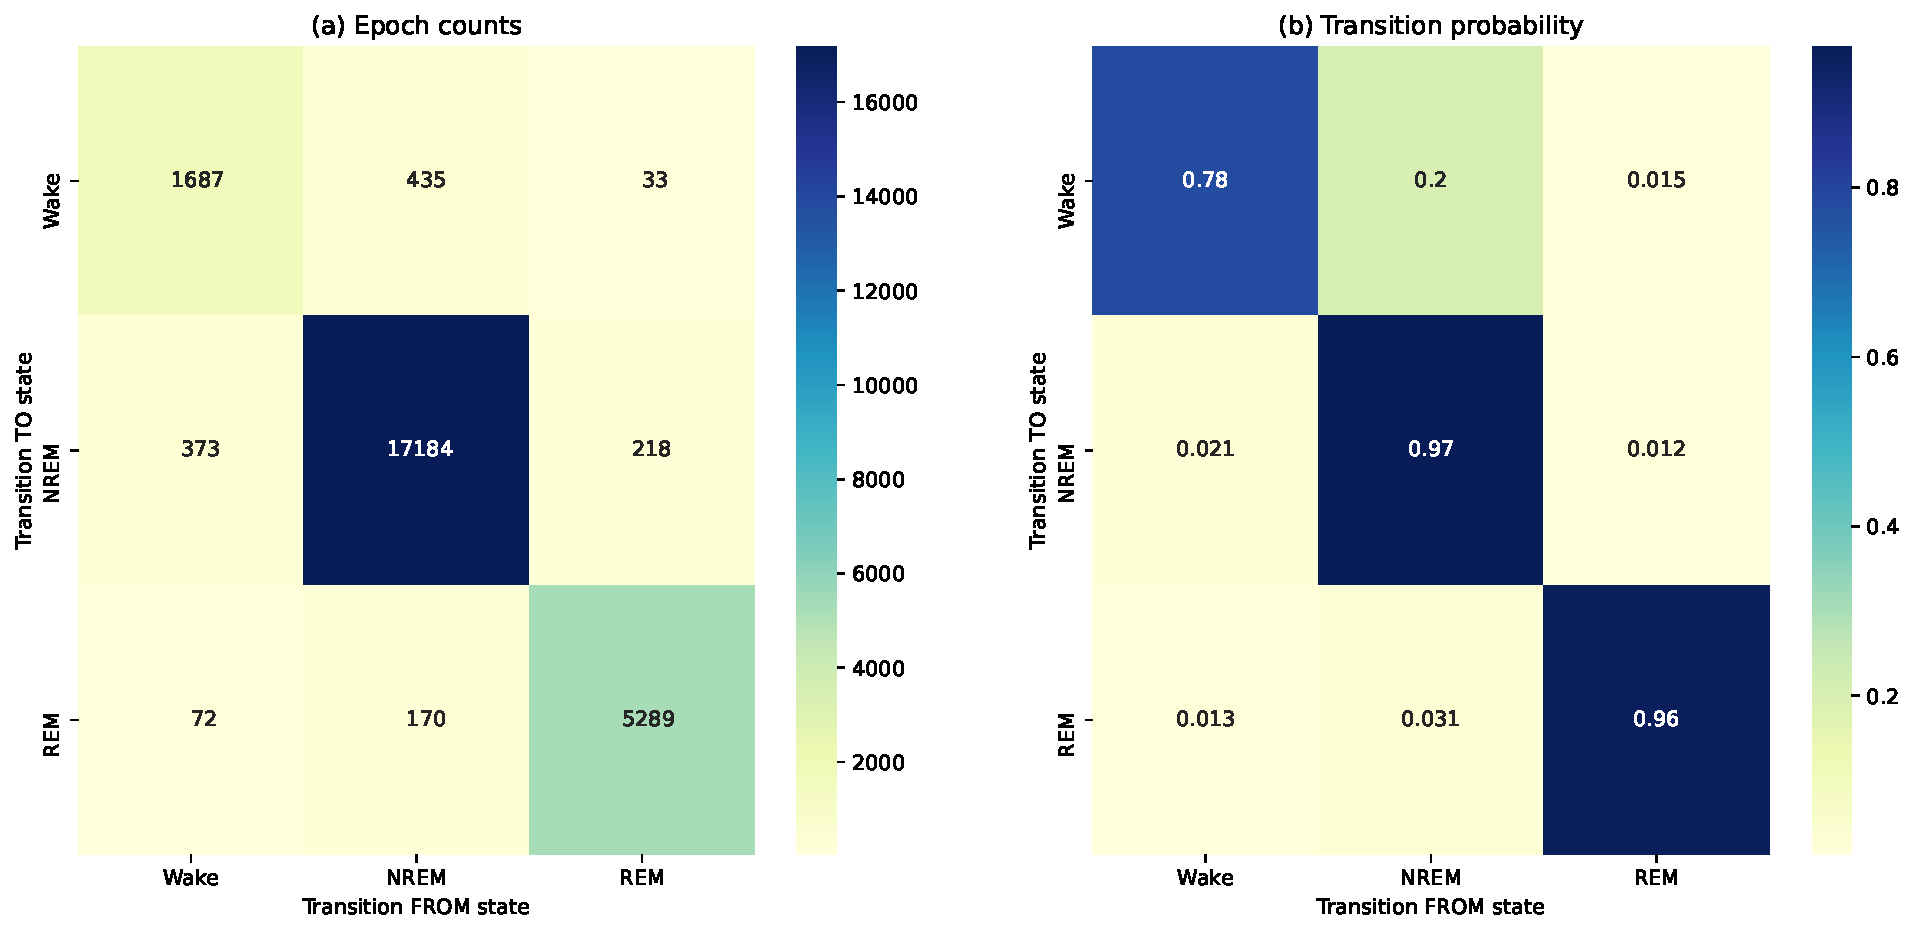
\includegraphics[width=1.\textwidth]{figures/sleep_stage_transitions.pdf}
%\label{fig:sleep_stage_transitions}
%\caption{Comparison of the subject-level classification accuracies across different models.}
%\end{figure}



\subsection{State-space model} One of the shortcomings of the baseline modeling approach is that they treat each epoch of sleep in isolation. This yields ``blips'' of sleep stages and ignores temporal correlations in the dataset \footref{dataurl}. As a new work, we considered state-space methods based on recurrent neural networks (RNNs) that can incorporate latent temporal structure into the predictive model. In terms of modeling framework, the current work is similar to \citet{radha2019sleep,haghayegh2021deep} that utilize deep neural networks for sleep stage classification. The RNN model chosen consists of a GRU block \citep{cho2014learning} mapping observed classification inputs to latent dynamics space. The latent space dynamics are then mapped to a fully connected block with one hidden layer, followed by the softmax classification layer. The latent units in the model can incorporate historical information from the input sequence. 


\subsection{Training setup} The modeling dataset consists of five feature sequences and one classification target sequence for 31 subjects. The full dataset was split into 8 training/testing sets with 30\% subjects selected for testing at random. For baseline classification models, we selected the best-performing parameters based on grid search using the training split. For RNN models, to avoid overfitting, the training dataset was further divided into train/validation splits randomly, and validation loss was used for early stopping. We used negative log-likelihood as the objective function for all models under consideration.


%\begin{figure}[t]
%	\centering
%	\begin{tikzpicture}[shorten >=1pt]
%		\tikzstyle{observable}=[draw,shape=circle,fill=gray]
%		\tikzstyle{hidden}=[draw,shape=circle,minimum size=1.15cm]
%		\tikzstyle{block}=[draw,shape=rectangle,minimum width=1.5cm,minimum height=1.5cm]
%		\node[observable](x1) at (0,0){$x_t$};
%		\node at (0,1){\vdots};
%		\node at (2,3.5){\vdots};
%		\node at (4,1){\vdots};	
%		\node[block](gru) at (2,0){GRU}; 			
%		\node[hidden](h0) at (2,2){$h_{t-1}$};
%		\node[hidden](h1) at (2,0){$h_t$};
%		\node[observable](y1) at (4,0){$y_t$};
%		\draw[->] (x1) -- (h1);
%		\draw[->] (h0) -- (h1);
%		\draw[->] (h1) -- (y1);
%	\end{tikzpicture}
%\end{figure}

\section{Results}
We considered two baseline models logistic regression and random forests along with a new RNN model in this study. We trained models on 8 different training/testing splits independently and report the average values for different performance metrics in this section. Figure \ref{fig:8000685_prediction} compares the ground truth sequence to the label sequence predicted by different classification models for the test subject \texttt{8000685}.


\begin{figure}
\centering
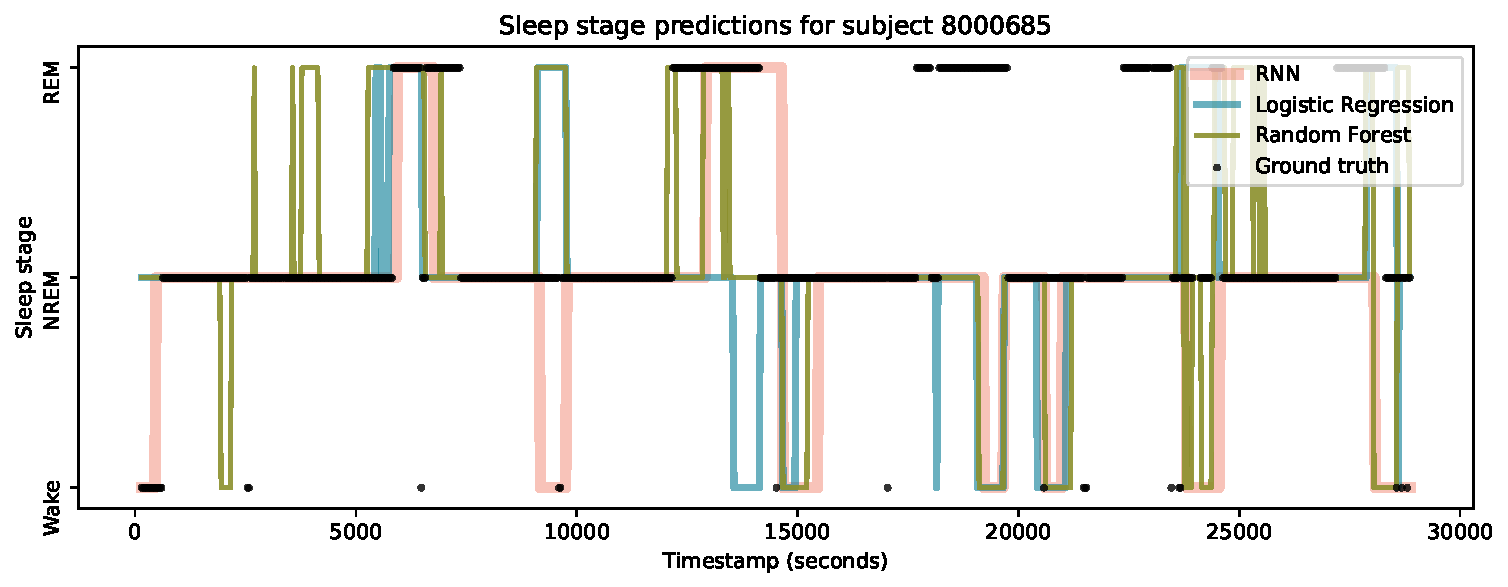
\includegraphics[width=\textwidth]{figures/8000685_predictions.pdf}
\caption{Visualization of the model predictions for subject  \texttt{8000685} for three different models RNN classifier, logistic regression and random forest as compared to the ground truth. All the models give misclassified assignments without a distinct misclassification pattern.}
\label{fig:8000685_prediction}
\end{figure}

The overall classification performance in terms of different metrics is reported in Table \ref{table:overall_classification}. As seen from the table, all the models learn to classify three different sleep stages at more than 65\% accuracy score. The results for baseline classifiers are similar to those reported by \cite{walch2019} on the dataset. The logistic regression classifier performs the best in terms of overall accuracy. However, the overall accuracy score might not be the best metric of choice for assessing the classification performance in the case of the imbalanced dataset as the metric is biased towards the majority label in terms of the number of observations. Figure \ref{fig:subject_level_accuracy} shows distribution of  classification agreements across sleep stages for different classifiers. From the figure, we can see that all three sleep stages are predicted with almost similar accuracy in the case of RNN and random forest models, whereas the logistic regression is more biased towards the dominant NREM class. In addition, the confusion matrix (normalized by the number of observations in the dataset) reported in Figure \ref{fig:confusion_matrix} indicates that while the logistic regression model predicts the majority class NREM accurately, it fails to predict the REM and Wake classes accurately.  


We can instead consider assessing the classification performance based on the balanced accuracy score, which computes the average recall obtained on each class. From Table \ref{table:overall_classification}, we can see that the RNN model gives a better-balanced accuracy score as compared to the other baseline methods. In addition, Figure \ref{fig:one_vs_rest_roc_comparison} shows the one-vs-rest ROC scores for all three classification models. As shown in the figure, the RNN model performs better than the other baseline models, the result of which is also quantified in terms of area-under-the-curve (AUC) score reported in Table \ref{table:overall_classification}. In addition, we also included Cohen's kappa statistic \citep{cohen1960coefficient} that takes into account the potential for classification agreement to happen by chance. In terms of this static, the RNN model again outperforms the other baseline models as shown in Table \ref{table:overall_classification}. 


\begin{table*}[t]
\centering
\caption{Classification metrics for test subjects. The best values bolded. ($\uparrow$): higher is better, ($\downarrow$) lower is better}
\resizebox{0.9\textwidth}{!}{
\begin{tabular}{l c c c c}
\toprule
Method & Acuracy ($\uparrow$) & Balanced acuracy ($\uparrow$)  & ROC AUC ($\uparrow$) & Cohen $\kappa$ ($\uparrow$) \\
\midrule
RNN & 0.676 & \textbf{0.685} &  \textbf{0.851} & \textbf{0.418} \\
Logistic Regression & \textbf{0.718} & 0.573 &  0.786 & 0.359 \\
Random Forest & 0.666 & 0.593 &  0.796 & 0.342\\
\bottomrule
\end{tabular}
}
\label{table:overall_classification}
\end{table*}


\begin{figure}
\centering
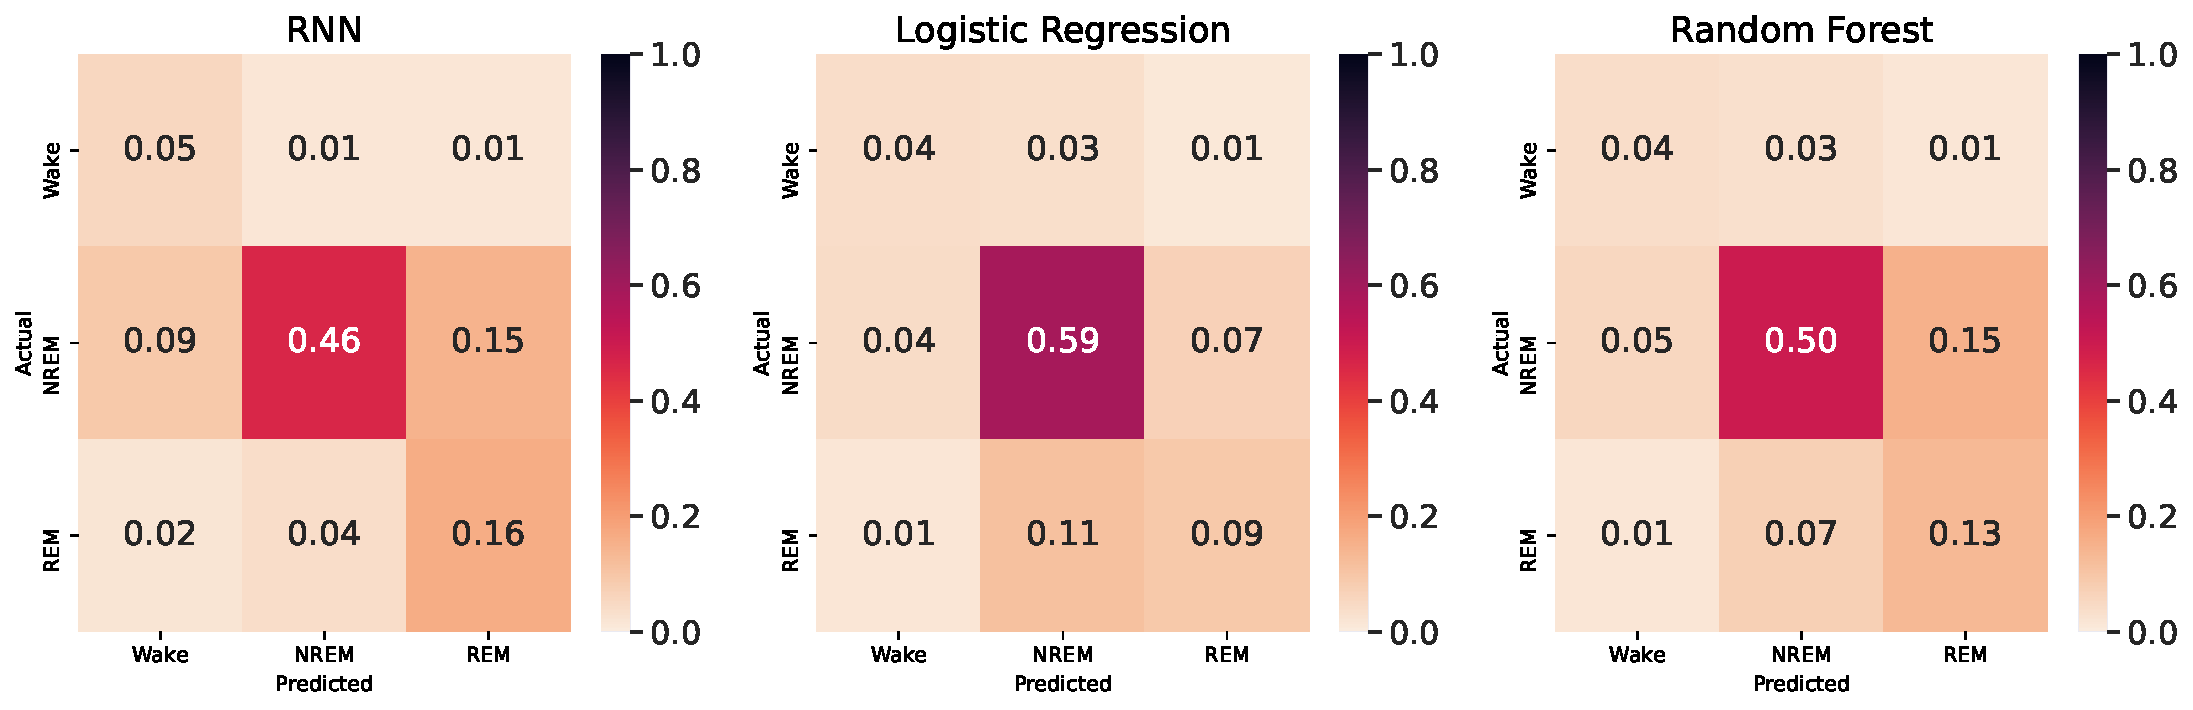
\includegraphics[width=\textwidth]{figures/confusion_matrix.pdf}
\caption{Confusion matrix (normalized by the number of observations) for different models.}
\label{fig:confusion_matrix}
\end{figure}






In addition, we follow the multi-class sleep stage classification analysis of \citep{walch2019} and report the results in this work. This analysis applies two thresholds to the class probabilities predicted by the classification models. The first threshold was applied to keep the false positive rate for the Wake class at 60\%. A second threshold was then applied to those epochs not scored as Wake under the first threshold. This second threshold was chosen to maintain the REM and NREM class accuracies as close to equal as possible. As noted by \citep{walch2019}, this method of analyzing classification models requires the
true labels for testing sets. Hence this analysis should 
be only considered for understanding the model performance
when the ground truth is known. The quantitative results from this analysis are reported in Table \ref{table:threshold_classification}. From the numbers, we can see that the classifier RNN model can accurately classify NREM and REM stages with 72\% accuracy which is more than 10\% improvement over other baseline methods. In terms of the Cohen $\kappa$ statistic, the RNN again outperforms the baseline classifiers. 

 
\begin{table*}[t]
\centering
\caption{Classification metrics for test subjects based on binary search. The best values bolded. ($\uparrow$): higher is better, ($\downarrow$) lower is better}
\resizebox{0.9\textwidth}{!}{
\begin{tabular}{l c c c c c}
\toprule
Method & Wake correct $\uparrow$ & NREM correct $\uparrow$ & REM correct $\uparrow$ & Cohen $\kappa$
$\uparrow$  \\
\midrule
RNN & 0.600 &  \textbf{0.720} & \textbf{0.720} & \textbf{0.465} \\
Logistic Regression & 0.600 &  0.633 & 0.631  & 0.303 \\
Random Forest & 0.600 &  0.610 & 0.609  & 0.333 \\
\bottomrule
\end{tabular}
}
\label{table:threshold_classification}
\end{table*}

\begin{figure}
\centering
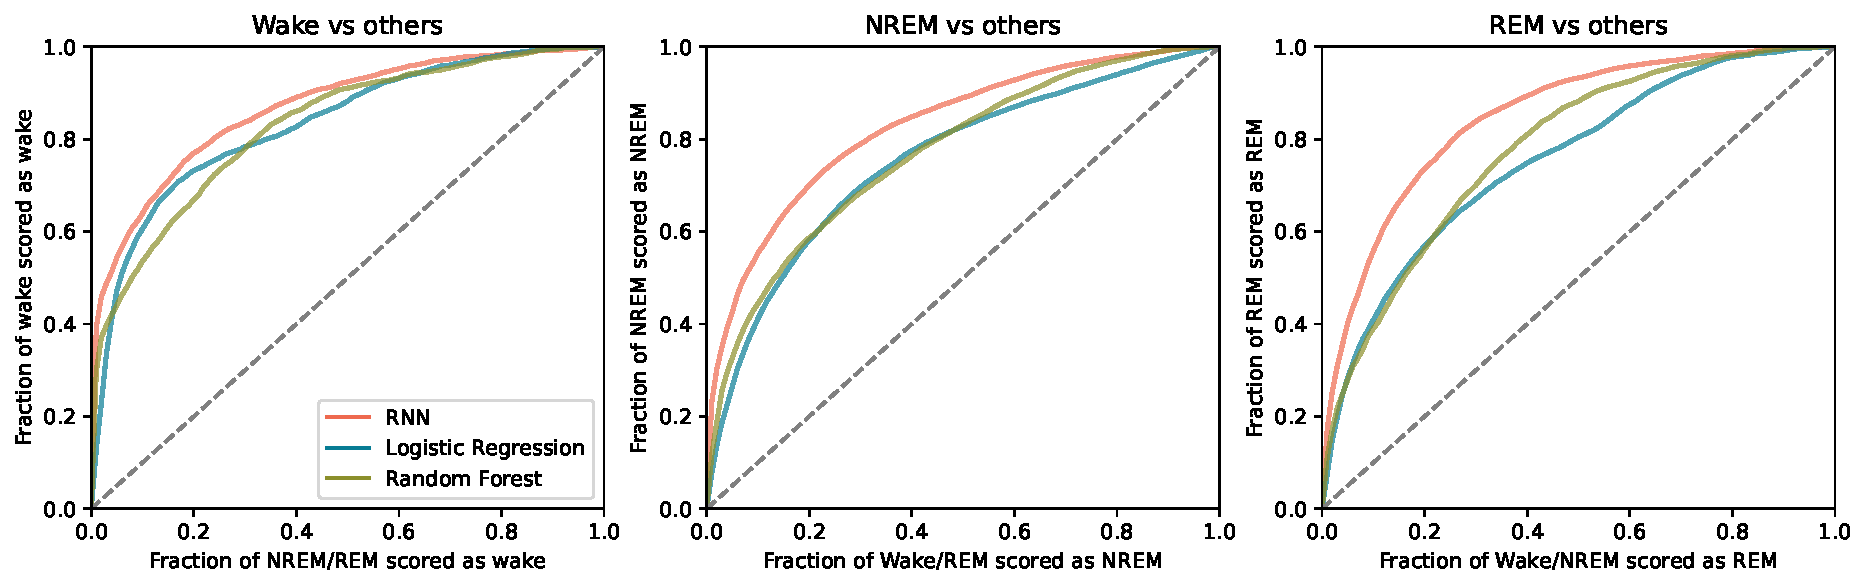
\includegraphics[width=\textwidth]{figures/one_vs_rest_roc_comparison.pdf}
\caption{One vs rest ROC score comparison  for sleep stage classification problem across different models. While the most prominent NREM state is classified almost equally well by all three models, RNN-based model performs better compared to the baselines on REM and Wake stages.}
\label{fig:one_vs_rest_roc_comparison}
\end{figure}


\begin{figure}
\centering
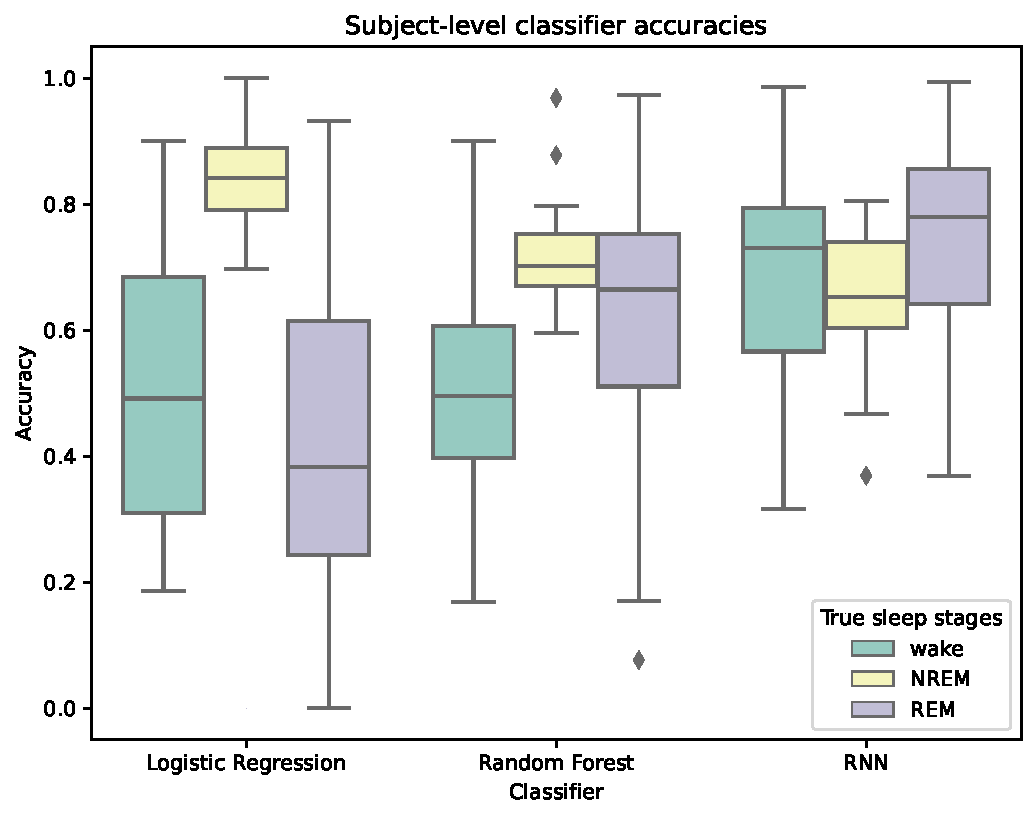
\includegraphics[width=0.6\textwidth]{figures/subject_level_accuracy.pdf}
\caption{Comparison of the subject-level classification accuracies across different models. Logistic regression gives good accuracy on the NREM majority class, while gives poor accuracy on REM and Wake. In contrast, random forest and RNN classifiers provide almost equal accuracy on all three classes, with RNN performing best in terms of average accuracy.}
\label{fig:subject_level_accuracy}
\end{figure}

\section{Conclusion and discussion}
We considered the problem of estimating sleep stages based on physiological observations and a proxy feature for circadian rhythm. In particular, the study explores the possibility of identifying sleep stages based on motion and heart rate measurements from a wrist wearable device. While the previous methods on the dataset under study modeled each sleep epoch isolation, such modeling methodology ignores the temporal correlations in the sleep data. As an attempt at improving the sequence classification modeling, we considered a state-space method based on RNNs in this study. The results show that incorporating such temporal structure into the model can help in improving the sleep stage classification problem. 

In this work, we considered a straightforward implementation of RNNs for modeling temporal dynamics in the sleep data. From a machine learning modeling perspective, there are multiple rooms for improvement. Within the current modeling framework, one could consider deriving more informative features such as the circadian feature based on the ambulatory data as defined in \citet{walch2019}. 

The dataset under study consists of raw measurements at irregular time intervals. In this work, we generated aggregated raw data to uniform time intervals (sleep stage epochs) by generating features corresponding to the first and second-order statistics (mean and variation respectively). However, the higher-order information could be lost because of this aggregation, which might be useful for predictive modeling. A possible future direction could be to develop models that can handle irregularly sampled time series data \citep{sun2020review}. The dataset understudy had only one night of observation for a total of 31 subjects, which can be quite limited. Another line of extension could be to consider probabilistic approaches that could provide better generalization under the limited number of observations \citep{fortunato2017bayesian}.  

In this current work, we considered the utilization of heart rate and motion measurements for predicting sleep stages. The state transitions throughout a sleep episode are also known to generate variations in other observables such as body temperature and respiration rates among others. One could incorporate such features in the predictive modeling that are tracked in many consumer wearable devices. In addition, we considered a single predictive model at the population level with an assumption that the features capture sufficient individual-level information. Inclusion of additional relevant information such as demographic parameters could be essential for generalization to wider populations.  



\bibliographystyle{plainnat}
\bibliography{references}

\end{document}

